\chapter{Graph Laplacian Embedding}
In the following section, an introduction to manifolds and the GL embedding is given.

\section{Manifolds}
\label{sec:manifolds}

% \textbf{TODO:
% it maps Rd to RD, if d<D. 
% In our case, it map an angle in S1 (subset of R) to something in RM. The circle S1, is 1 dimensional, 
% it depends only on 1 parameter, and can be represented in R2 like you did. 
% I thinks (not 100 of sure of that right now) that the  rotation group is a manifold, 
% it maps 1d parameter (rotation angle) to some rotation operator (which is high dimensional)
% we don't calculate manifold. 
% Diffusion maps (or graph Laplacian embedding) are a way to map high dimensional dataset to low dimensional one. 
% When the data points are sampled from a manifold, the GL embedding is closely related to the manifold itself.
% We can expect the GL embedding to share property of the original manifold, such as preservation of distances between points}

The manifold assumption is a popular assumption for high-dimensional datasets.
For a given dataset in high-dimension, one can assume that data points are samples drawn from a low-dimensional manifold,
that embeds the high-dimensional space. 
Therefore, if underlying manifold can be approximated, a dimensionality reduction
is established as one can embed data points in the low-dimensional manifold space.
There is a complete area of research devoted to this manifold assumption called Manifold Learning~\cite{ManifoldLearning}.

For high-dimensional data Euclidean distances are not meaningful in the sense that they will not capture similar data points well. 
GL can be used to compute a low-dimensional embedding which can map from high-dimensional space to the low-dimensional space.
In the low-dimensional space, Euclidean distances make sense again. 


\paragraph{Definition:}
Let manifold $M$ be defined as $\mathcal{M} = \{ f(x), f \in C^K, f: \mathbb{R}^D \to \mathbb{R}^d \}$.
In this Thesis, only $C^k$ differentiable d-dimensional manifolds defined by $\mathcal{M}$ are considered. 
When $d \ll D$, the manifold defines a low-dimensional embedding, which maps from high-dimensional space 
$\mathbb{R}^D$ to low-dimensional space $\mathbb{R}^d$.

Let's give two popular examples of manifolds, namely the \textit{circle} and the \textit{sphere}.
The circle is a 1D manifold, where $d=1$ and $D=2$. A sphere is a 2D manifold with $d=2$ and $D=3$.
In Figure~\ref{fig:circle_sampling}, 200 samples are drawn from a uniform distribution of the unit-circle manifold
and in Figure~\ref{fig:sphere_sampling}, 800 samples are drawn from a uniform distribution of the unit-sphere manifold,
as well as the sphere itself.



\begin{figure}[H]
    \captionsetup[subfigure]{justification=centering}
    \centering
    \begin{subfigure}[t]{0.4\textwidth}
        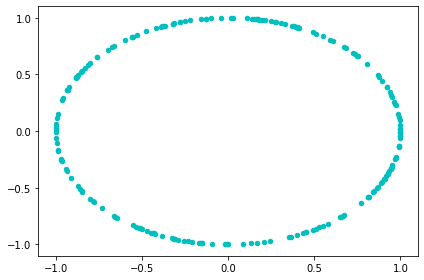
\includegraphics[width=\textwidth]{circle_sampling.png}
        \caption{Samples drawn for the unit-circle.}
        \label{fig:circle_sampling}
    \end{subfigure}\hfill
    \begin{subfigure}[t]{0.4\textwidth}
      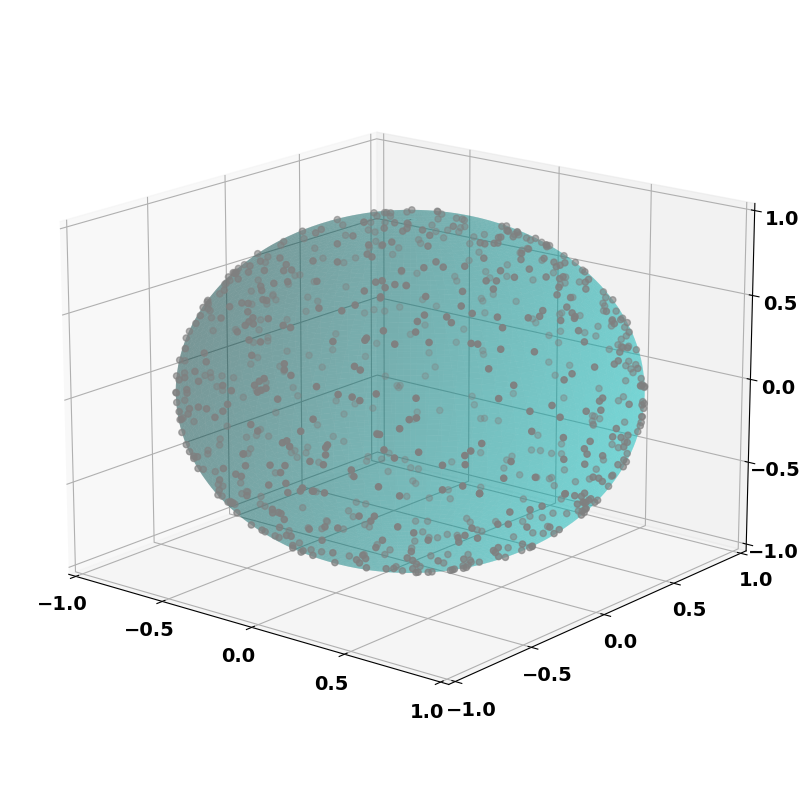
\includegraphics[width=\textwidth]{sphere_sampling.png}
      \caption{Samples drawn for the unit-sphere.}
      \label{fig:sphere_sampling}
    \end{subfigure}\hfill
    \caption{Samples drawn from a 1D and 2D manifold.}
  \end{figure}


\paragraph{GL embedding}
\label{sec:manifold_calculation}
A low-dimensional embedding of a dataset can be computed with GL by the following:

\begin{enumerate}
    \item Construct the k-NN graph from dataset
    \item Calculate the GL
    \item Extract the second, third (and fourth) smallest eigenvectors
\end{enumerate}

Another popular algorithm for calculating a low-dimensional embedding is diffusion maps~\cite{diffusionMaps}, 
which is a non-linear approach using GL.
Vector diffusion maps~\cite{vectorDiffusionMaps} generalize the concept of diffusion maps for vector fields.
Multi-frequency vector diffusion maps~\cite{multiDiffusionMaps} 
can be seen as an extension to vector diffusion maps, which works well even on highly noisy environments.
\citet{cryoEmMutliDM} successfully applied multi-frequency vector diffusion Maps in cryo-EM setting,
 where it was used for denoising observations.


\subsection{Embedding Quality}
\label{sec:embedding_quality}

Finding a good embedding is not trivial and in our case, the embedding is dependent on $k$ during graph construction
as well as parameter $\theta$, $s$ and $\eta$.

$k$ is an important parameter for building up a graph. If set too low, neighbors
do not capture similar data well as too few nodes are connected. 
Further, if k is set too high, strength of a neighbor 
is weakened and data is not well explained.
In Figure~\ref{fig:clean_manifolds}, the GL embedding computed from clean sinogram and $k$ from 2 to 10 is illustrated.
From $k \leq 4$ the GL embedding approximates a circle and with $k >  4$ it moves further away from the circle. 


\begin{figure}[H]
    \captionsetup[subfigure]{justification=centering}
    \centering
    \begin{subfigure}[t]{0.45\textwidth}
        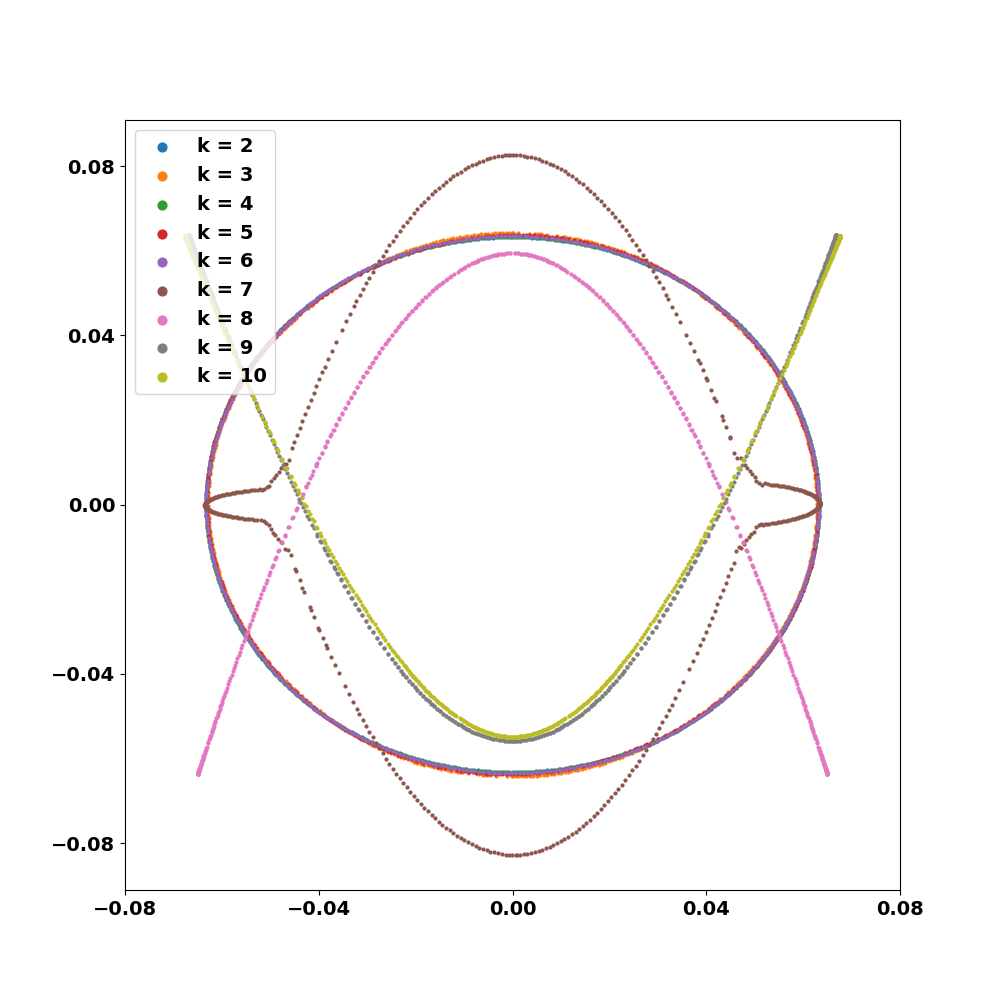
\includegraphics[width=\textwidth]{phaton_clean_manifold_kdifferent.png}
        \caption{Clean sinogram GL embeddings for different $k$.}
        \label{fig:clean_manifolds}
    \end{subfigure}\hfill
    \begin{subfigure}[t]{0.45\textwidth}
      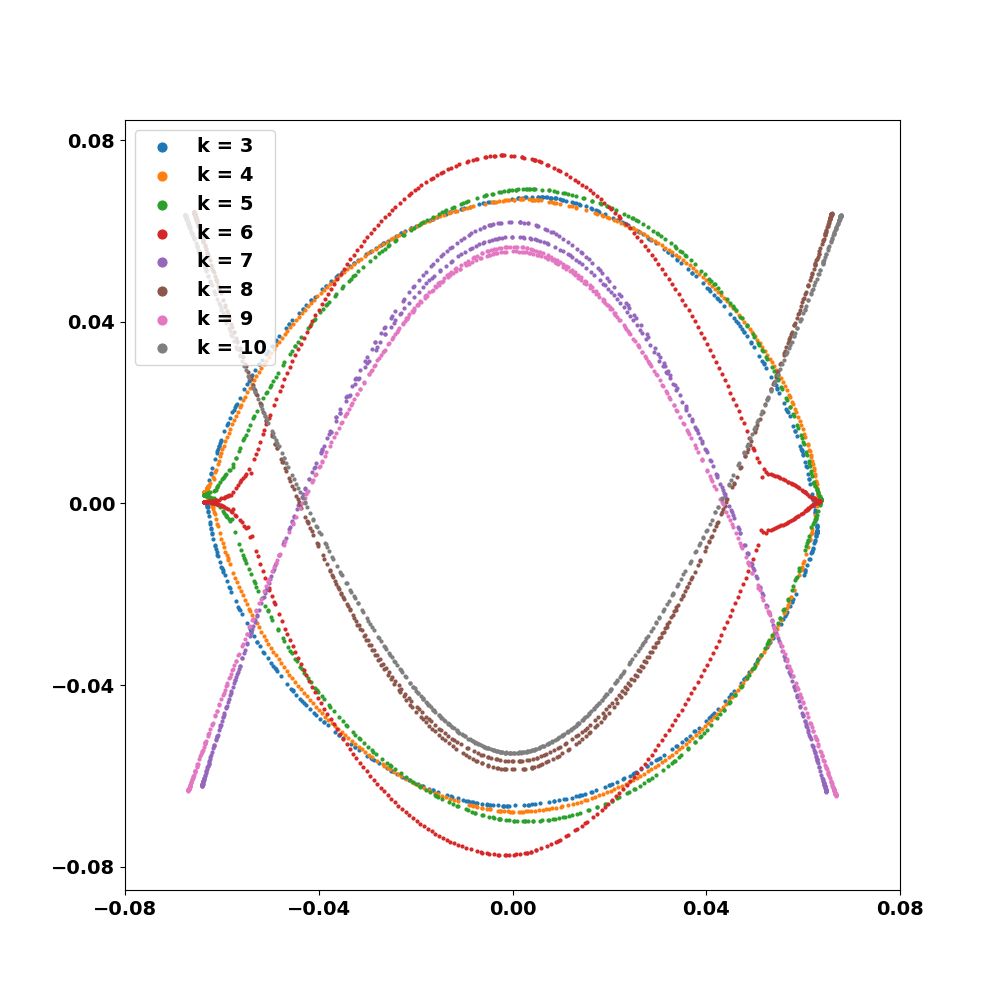
\includegraphics[width=\textwidth]{phaton_noisy_manifold_kdifferent.png}
      \caption{Noisy sinogram GL embeddings for different $k$.}
      \label{fig:noisy_manifolds}
    \end{subfigure}\hfill
    \caption{Shepp-Logan phantom sinogram GL embeddings for different $k$.}
  \end{figure}

If data is noisy, it is expected to be harder to construct a meaningful GL embedding, as some connections within
the graph will be noisy. This is exactly what is illustrated in Figure~\ref{fig:noisy_manifolds}, where 
different GL embedding for noisy sinogram (SNR=20dB) and k from 3 to 10 are illustrated.
GL embedding can never express data with a perfect circle. As noise is chosen rather moderate, GL embedding has still some 
power to express underlying data and is expected to decrease, if noise is increased.


Further, when observing a sinogram, $\theta$ defines how many observations (straight lines) are drawn
and $dim(s)$ defines the amount of sampling points. Both have great impact to expressiveness of our sinogram.
In Figure~\ref{fig:clean_manifold_200} GL embedding with $\theta \in \mathbb{R}^{200}$ and k=6 is illustrated
for clean sinogram. It looks like 6 are too many neighbors, as the perfect circle cannot be established anymore.
But, if $\theta$ is increased to $\theta \in \mathbb{R}^{500}$, more nodes are available to choose good neighbors from
and a circle can be established (Figure~\ref{fig:clean_manifold_500}).

\begin{figure}[H]
    \captionsetup[subfigure]{justification=centering}
    \centering
    \begin{subfigure}[t]{0.45\textwidth}
        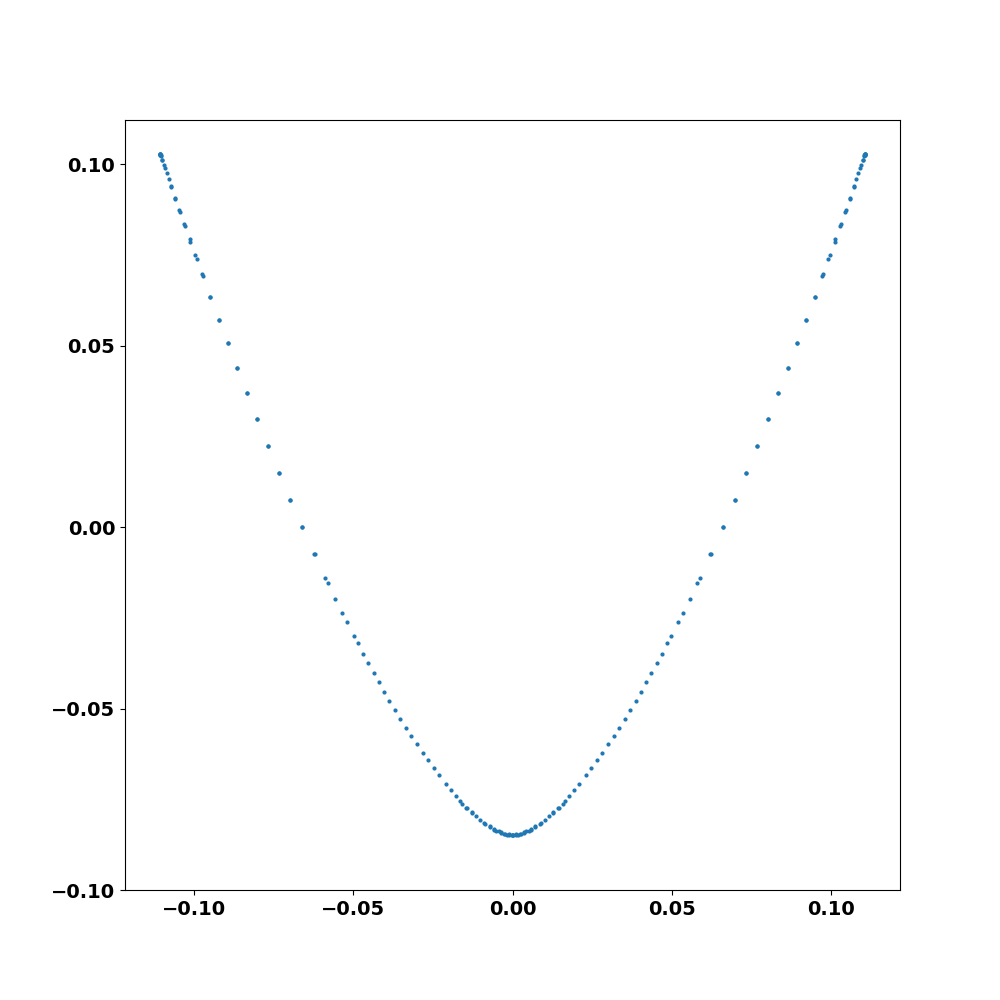
\includegraphics[width=\textwidth]{phaton_clean_manifold_200_k6.png}
        \caption{Clean sinogram GL embedding, $k = 6$ and 200 samples}
        \label{fig:clean_manifold_200}
    \end{subfigure}\hfill
    \begin{subfigure}[t]{0.45\textwidth}
      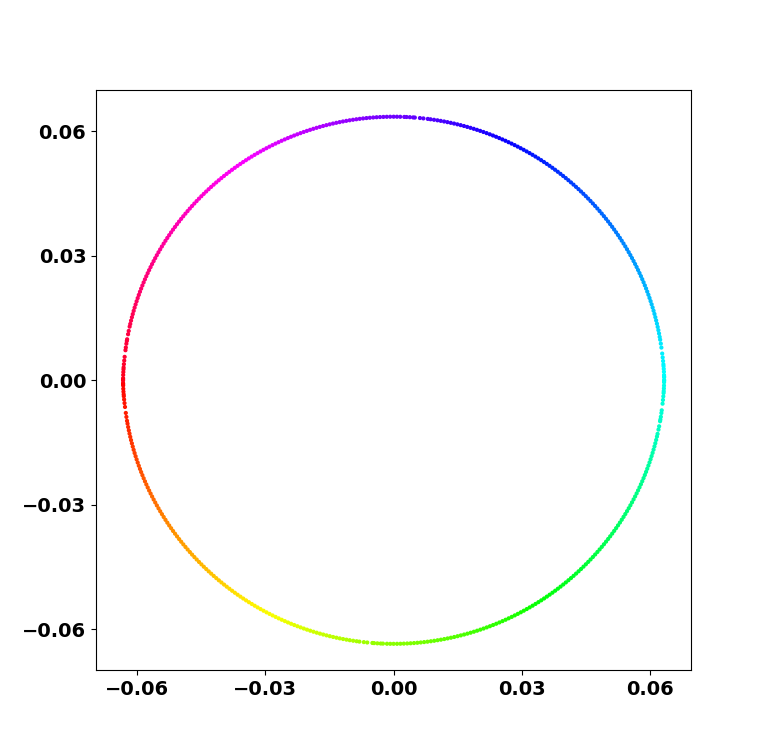
\includegraphics[width=\textwidth]{phaton_clean_manifold_500_k6.png}
      \caption{Clean sinogram GL embedding, $k = 6$ and 500 samples.}
      \label{fig:clean_manifold_500}
    \end{subfigure}\hfill
    \caption{Shepp-Logan phantom sinogram GL embeddings: Importance of number of samples}
  \end{figure}


Moreover, the number of sampling points is important as well.
For more sampling points it is expected to be harder to come up with good neighbors (fixing k and number of samples),
as more data needs to be explained with the same amount of neighbors. It is more likely, that nodes are connected wrongly.
This can be seen in Figure~\ref{fig:clean_manifold_res200} and Figure~\ref{fig:clean_manifold_res400}, where with $dim(s) = 200$,
the perfect circle can be established and with $dim(s) = 400$, not anymore (by same parameter $k = 6$ and $\theta \in \mathbb{R}^{500}$).

\begin{figure}[H]
    \captionsetup[subfigure]{justification=centering}
    \centering
    \begin{subfigure}[t]{0.4\textwidth}
        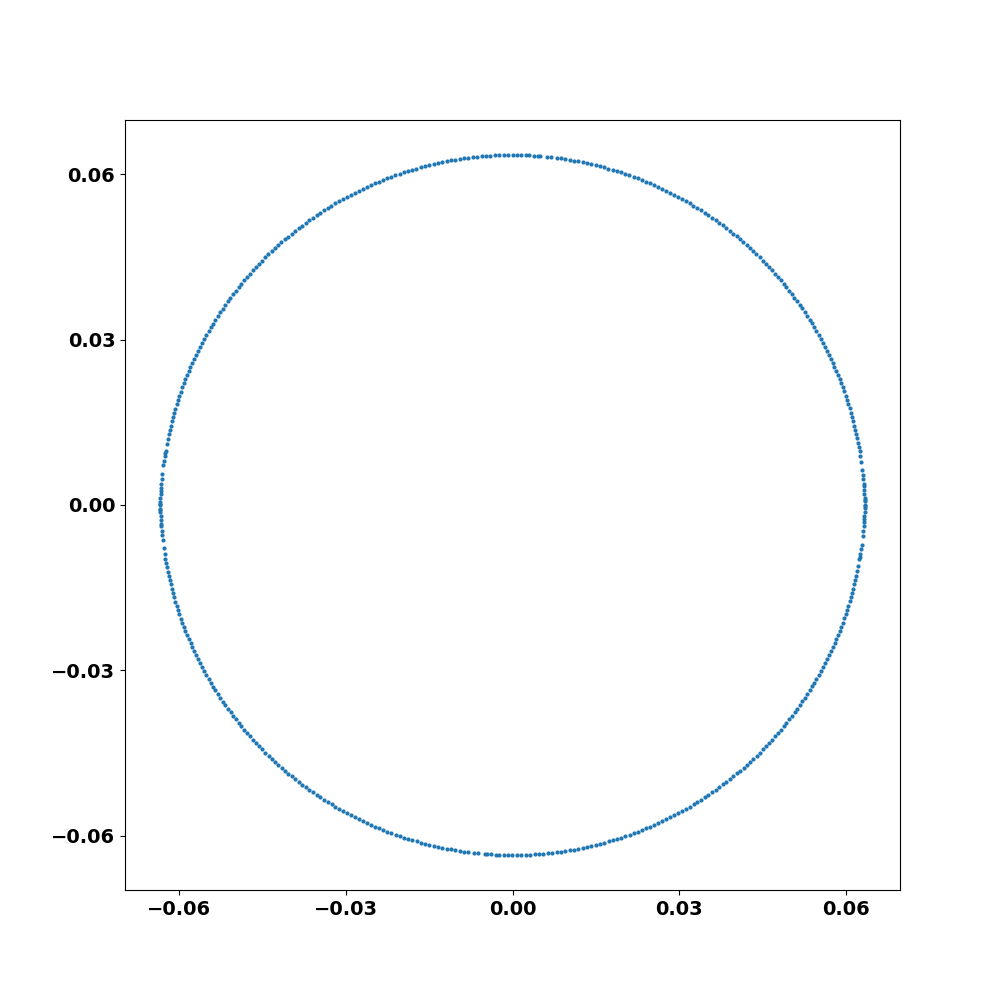
\includegraphics[width=\textwidth]{phaton_clean_manifold_res_200_k6.png}
        \caption{Clean sinogram GL embedding, $k = 6$ and $dim(s)=200$.}
        \label{fig:clean_manifold_res200}
    \end{subfigure}\hfill
    \begin{subfigure}[t]{0.4\textwidth}
      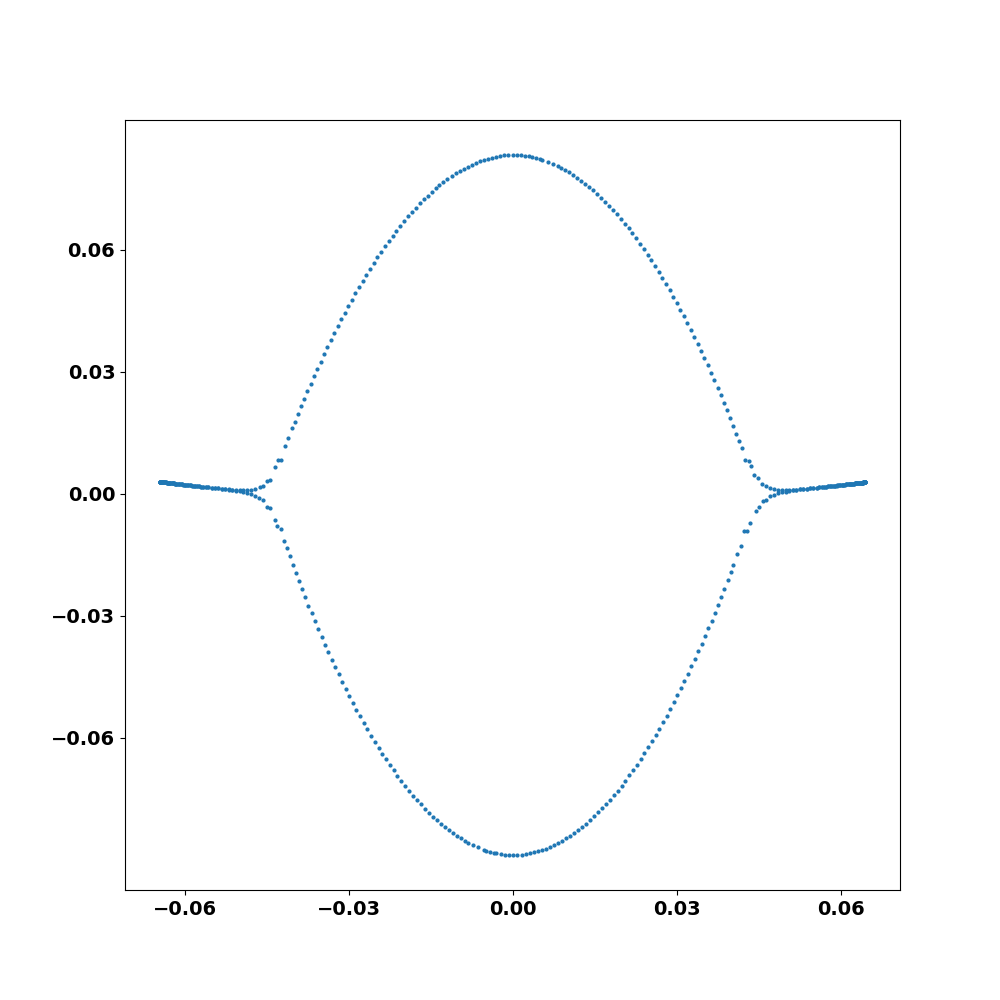
\includegraphics[width=\textwidth]{phaton_clean_manifold_res_400_k6.png}
      \caption{Clean sinogram GL embedding, $k = 6$ and $\dim(s)=400$.}
      \label{fig:clean_manifold_res400}
    \end{subfigure}\hfill
    \caption{Shepp-Logan phantom sinogram GL embeddings: Importance of sample dimension.}
  \end{figure}

\begin{tcolorbox}[colback=red!5!white,colframe=red!75!black]
    Since the GL embedding is sensitive to $k$, it is best practice to try different values in order to find the best GL-manifold.
\end{tcolorbox}





